\section{Ops\_\-Basic Class Reference}
\label{classOps__Basic}\index{Ops_Basic@{Ops\_\-Basic}}
This class supplies basic functions for getting access to neural netwoks stored in chromosome. 


{\tt \#include $<$Ops\_\-Basic.h$>$}

Inheritance diagram for Ops\_\-Basic::\begin{figure}[H]
\begin{center}
\leavevmode
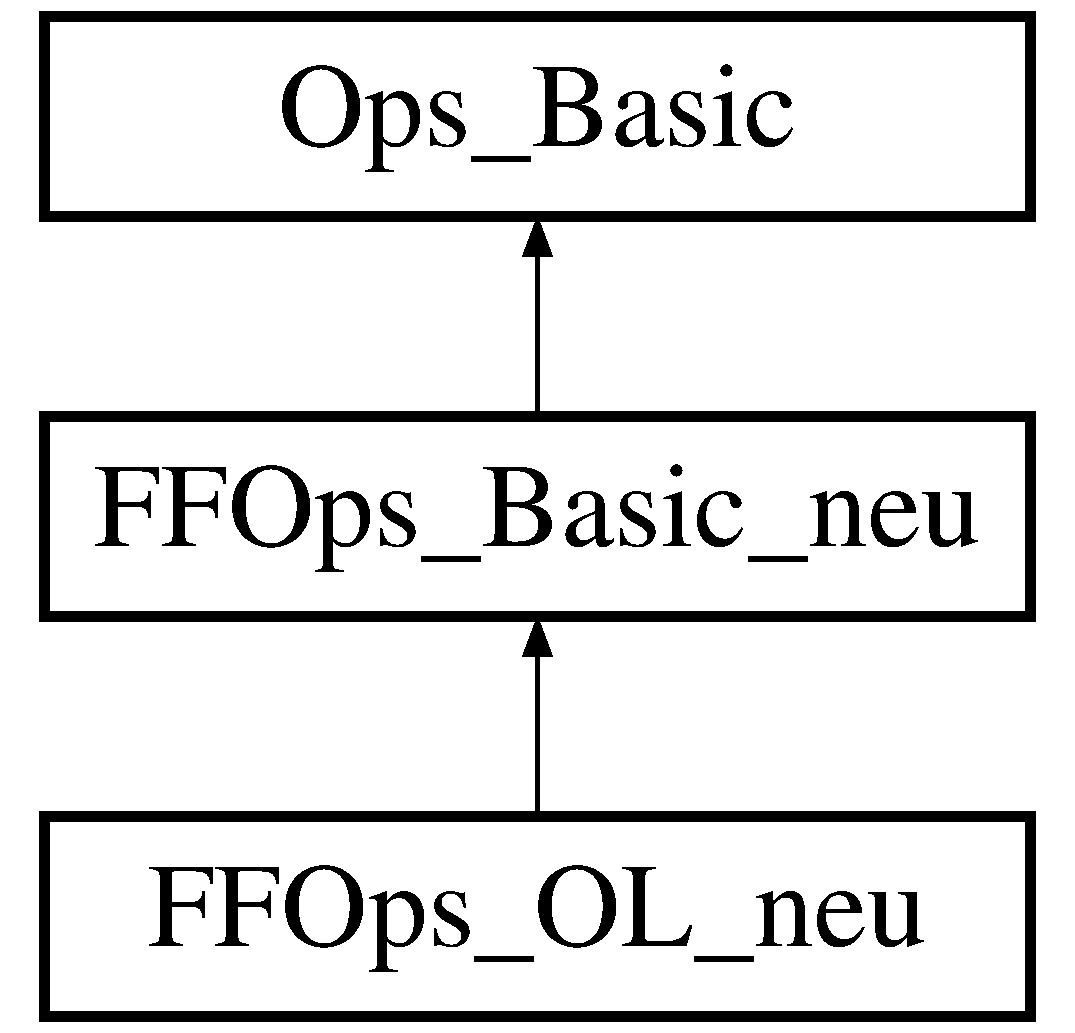
\includegraphics[height=3cm]{classOps__Basic}
\end{center}
\end{figure}
\subsection*{Public Methods}
\begin{CompactItemize}
\item 
Individual {\bf create\-Empty} (const unsigned n\-In, const unsigned n\-Hid, const unsigned n\-Out, const unsigned n\-Delay)
\begin{CompactList}\small\item\em Creat an new individual for representing a network.\item\end{CompactList}\item 
void {\bf init\-Weights} (Individual \&Ind, double low, double high)
\begin{CompactList}\small\item\em Initialize the weights randomly within a given interval.\item\end{CompactList}\item 
\index{getConnections@{getConnections}!Ops_Basic@{Ops\_\-Basic}}\index{Ops_Basic@{Ops\_\-Basic}!getConnections@{getConnections}}
Array$<$ int $>$ {\bf get\-Connections} (Individual \&Ind)\label{classOps__Basic_a2}

\begin{CompactList}\small\item\em Return the connection matrix of three dimensional.\item\end{CompactList}\item 
Array$<$ int $>$ {\bf get\-Connections} (Individual \&Ind, unsigned entry)
\begin{CompactList}\small\item\em Returns the connection matrix of two dimensional of a given time.\item\end{CompactList}\item 
Array$<$ double $>$ {\bf get\-Weights} (Individual \&Ind)
\begin{CompactList}\small\item\em Return the weights of the network.\item\end{CompactList}\item 
Array$<$ double $>$ {\bf get\-Weights} (Individual \&Ind, unsigned entry)
\begin{CompactList}\small\item\em Returns the weights of a given time.\item\end{CompactList}\item 
unsigned {\bf get\-NIn} (Individual \&Ind)
\begin{CompactList}\small\item\em Return the number of input neurons.\item\end{CompactList}\item 
unsigned {\bf get\-NHid} (Individual \&Ind)
\begin{CompactList}\small\item\em Return the number of hidden neurons.\item\end{CompactList}\item 
unsigned {\bf get\-NOut} (Individual \&Ind)
\begin{CompactList}\small\item\em Return the number of output neurons.\item\end{CompactList}\item 
unsigned {\bf get\-NDelay} (Individual \&Ind)
\begin{CompactList}\small\item\em Return the time index of the network.\item\end{CompactList}\item 
unsigned {\bf get\-NParameter} (Individual \&Ind)
\begin{CompactList}\small\item\em Return the number of all parameters contained in the network.\item\end{CompactList}\item 
\index{printNet@{printNet}!Ops_Basic@{Ops\_\-Basic}}\index{Ops_Basic@{Ops\_\-Basic}!printNet@{printNet}}
void {\bf print\-Net} (Individual \&Ind, string filename)\label{classOps__Basic_a11}

\begin{CompactList}\small\item\em Print the network structure and parameters to a file called {\tt filename}.\item\end{CompactList}\item 
void {\bf set\-Structure} (Individual \&Ind, const Array$<$ double $>$ \&w, unsigned entry)
\begin{CompactList}\small\item\em Replace the weights of a given time index with those provided.\item\end{CompactList}\item 
void {\bf set\-Structure} (Individual \&Ind, const Array$<$ double $>$ \&w)
\begin{CompactList}\small\item\em Replace all weights with those provided.\item\end{CompactList}\item 
void {\bf set\-Structure} (Individual \&Ind, const Array$<$ int $>$ \&c, unsigned entry)
\begin{CompactList}\small\item\em Replace the connections of a given time index with those provided.\item\end{CompactList}\item 
void {\bf set\-Structure} (Individual \&Ind, const Array$<$ int $>$ \&c)
\begin{CompactList}\small\item\em Replace connections with those provided.\item\end{CompactList}\item 
void {\bf jog\-Weights} (Individual \&Ind, const double stdv, double prob=1.0)
\begin{CompactList}\small\item\em Mutate the weights.\item\end{CompactList}\end{CompactItemize}
\subsection*{Protected Methods}
\begin{CompactItemize}
\item 
unsigned {\bf get\-NNeurons} (Individual \&Ind)
\begin{CompactList}\small\item\em Return the sum of neuron number in the network.\item\end{CompactList}\item 
void {\bf set\-NHid} (Individual \&Ind, unsigned n\-Hid)
\begin{CompactList}\small\item\em Change the number of hidden nodes according to a given number.\item\end{CompactList}\item 
void {\bf del\-Neuron} (Individual \&Ind, unsigned N)
\begin{CompactList}\small\item\em Delete a hidden neuron according to a given number.\item\end{CompactList}\item 
void {\bf ins\-Neuron} (Individual \&Ind, unsigned N)
\begin{CompactList}\small\item\em Insert a hidden neuron according to a given number.\item\end{CompactList}\item 
unsigned {\bf wheel\-Of\-Fortune} (Array$<$ double $>$ \&prob)
\begin{CompactList}\small\item\em randomly select a position in a probability matrix and return this position\item\end{CompactList}\end{CompactItemize}


\subsection{Detailed Description}
This class supplies basic functions for getting access to neural netwoks stored in chromosome.

Access operations include reading out the networks for mutation and again save the networks back to the chromosom. 



\subsection{Member Function Documentation}
\index{Ops_Basic@{Ops\_\-Basic}!createEmpty@{createEmpty}}
\index{createEmpty@{createEmpty}!Ops_Basic@{Ops\_\-Basic}}
\subsubsection{\setlength{\rightskip}{0pt plus 5cm}Individual Ops\_\-Basic::create\-Empty (const unsigned {\em n\-In}, const unsigned {\em n\-Hid}, const unsigned {\em n\-Out}, const unsigned {\em n\-Delay})}\label{classOps__Basic_a0}


Creat an new individual for representing a network.

Define a generic network by defining the number of input, hidden and output nodes. For generating recurrent networks, a parameter \par
 n\-Delay is also needed, whereas if feedforward networks are to be created, this should be fixed to 1. Finally, two three-dimensional matrices of the size {\tt n\-Delay$\ast$(n\-In+n\-Hid+n\-Out)$\ast$(n\-Delay+n\-In+n\-Hid+n\-Out)} will be generated.\begin{Desc}
\item[Parameters: ]\par
\begin{description}
\item[{\em 
n\-In:}]number of input nodes \item[{\em 
n\-Hid:}]number of hidden nodes \item[{\em 
n\-Out:}]number of output nodes \item[{\em 
n\-Delay:}]number of time delay \end{description}
\end{Desc}
\index{Ops_Basic@{Ops\_\-Basic}!delNeuron@{delNeuron}}
\index{delNeuron@{delNeuron}!Ops_Basic@{Ops\_\-Basic}}
\subsubsection{\setlength{\rightskip}{0pt plus 5cm}void Ops\_\-Basic::del\-Neuron (Individual \& {\em Ind}, unsigned {\em N})\hspace{0.3cm}{\tt  [protected]}}\label{classOps__Basic_b2}


Delete a hidden neuron according to a given number.

All hidden neurons are enumerated so that an arbitrary hidden neuron can be determined by an integer number. \begin{Desc}
\item[Parameters: ]\par
\begin{description}
\item[{\em 
Ind:}]individual to be processed \item[{\em 
N:}]the neuron to be deleted \end{description}
\end{Desc}
\index{Ops_Basic@{Ops\_\-Basic}!getConnections@{getConnections}}
\index{getConnections@{getConnections}!Ops_Basic@{Ops\_\-Basic}}
\subsubsection{\setlength{\rightskip}{0pt plus 5cm}Array$<$int$>$ Ops\_\-Basic::get\-Connections (Individual \& {\em Ind}, unsigned {\em entry})}\label{classOps__Basic_a3}


Returns the connection matrix of two dimensional of a given time.

\begin{Desc}
\item[Parameters: ]\par
\begin{description}
\item[{\em 
Ind:}]individual representing the network \item[{\em 
entry:}]time index for which connections should be returned. \end{description}
\end{Desc}
\index{Ops_Basic@{Ops\_\-Basic}!getNDelay@{getNDelay}}
\index{getNDelay@{getNDelay}!Ops_Basic@{Ops\_\-Basic}}
\subsubsection{\setlength{\rightskip}{0pt plus 5cm}unsigned Ops\_\-Basic::get\-NDelay (Individual \& {\em Ind})}\label{classOps__Basic_a9}


Return the time index of the network.

\begin{Desc}
\item[Parameters: ]\par
\begin{description}
\item[{\em 
Ind:}]individual representing the network to be accessed \end{description}
\end{Desc}
\index{Ops_Basic@{Ops\_\-Basic}!getNHid@{getNHid}}
\index{getNHid@{getNHid}!Ops_Basic@{Ops\_\-Basic}}
\subsubsection{\setlength{\rightskip}{0pt plus 5cm}unsigned Ops\_\-Basic::get\-NHid (Individual \& {\em Ind})}\label{classOps__Basic_a7}


Return the number of hidden neurons.

\begin{Desc}
\item[Parameters: ]\par
\begin{description}
\item[{\em 
Ind:}]individual representing the network to be accessed \end{description}
\end{Desc}
\index{Ops_Basic@{Ops\_\-Basic}!getNIn@{getNIn}}
\index{getNIn@{getNIn}!Ops_Basic@{Ops\_\-Basic}}
\subsubsection{\setlength{\rightskip}{0pt plus 5cm}unsigned Ops\_\-Basic::get\-NIn (Individual \& {\em Ind})}\label{classOps__Basic_a6}


Return the number of input neurons.

\begin{Desc}
\item[Parameters: ]\par
\begin{description}
\item[{\em 
Ind:}]individual representing the network to be accessed \end{description}
\end{Desc}
\index{Ops_Basic@{Ops\_\-Basic}!getNNeurons@{getNNeurons}}
\index{getNNeurons@{getNNeurons}!Ops_Basic@{Ops\_\-Basic}}
\subsubsection{\setlength{\rightskip}{0pt plus 5cm}unsigned Ops\_\-Basic::get\-NNeurons (Individual \& {\em Ind})\hspace{0.3cm}{\tt  [protected]}}\label{classOps__Basic_b0}


Return the sum of neuron number in the network.

\begin{Desc}
\item[Parameters: ]\par
\begin{description}
\item[{\em 
Ind:}]individual to access \end{description}
\end{Desc}
\index{Ops_Basic@{Ops\_\-Basic}!getNOut@{getNOut}}
\index{getNOut@{getNOut}!Ops_Basic@{Ops\_\-Basic}}
\subsubsection{\setlength{\rightskip}{0pt plus 5cm}unsigned Ops\_\-Basic::get\-NOut (Individual \& {\em Ind})}\label{classOps__Basic_a8}


Return the number of output neurons.

\begin{Desc}
\item[Parameters: ]\par
\begin{description}
\item[{\em 
Ind:}]individual representing the network to be accessed \end{description}
\end{Desc}
\index{Ops_Basic@{Ops\_\-Basic}!getNParameter@{getNParameter}}
\index{getNParameter@{getNParameter}!Ops_Basic@{Ops\_\-Basic}}
\subsubsection{\setlength{\rightskip}{0pt plus 5cm}unsigned Ops\_\-Basic::get\-NParameter (Individual \& {\em Ind})}\label{classOps__Basic_a10}


Return the number of all parameters contained in the network.

\begin{Desc}
\item[Parameters: ]\par
\begin{description}
\item[{\em 
Ind:}]individual representing the network to be accessed \end{description}
\end{Desc}
\index{Ops_Basic@{Ops\_\-Basic}!getWeights@{getWeights}}
\index{getWeights@{getWeights}!Ops_Basic@{Ops\_\-Basic}}
\subsubsection{\setlength{\rightskip}{0pt plus 5cm}Array$<$double$>$ Ops\_\-Basic::get\-Weights (Individual \& {\em Ind}, unsigned {\em entry})}\label{classOps__Basic_a5}


Returns the weights of a given time.

\begin{Desc}
\item[Parameters: ]\par
\begin{description}
\item[{\em 
Ind:}]individual representing the network \item[{\em 
entry:}]time index for which weights should be returned. \end{description}
\end{Desc}
\index{Ops_Basic@{Ops\_\-Basic}!getWeights@{getWeights}}
\index{getWeights@{getWeights}!Ops_Basic@{Ops\_\-Basic}}
\subsubsection{\setlength{\rightskip}{0pt plus 5cm}Array$<$double$>$ Ops\_\-Basic::get\-Weights (Individual \& {\em Ind})}\label{classOps__Basic_a4}


Return the weights of the network.

\begin{Desc}
\item[Parameters: ]\par
\begin{description}
\item[{\em 
Ind:}]individual representing the network \end{description}
\end{Desc}
\index{Ops_Basic@{Ops\_\-Basic}!initWeights@{initWeights}}
\index{initWeights@{initWeights}!Ops_Basic@{Ops\_\-Basic}}
\subsubsection{\setlength{\rightskip}{0pt plus 5cm}void Ops\_\-Basic::init\-Weights (Individual \& {\em Ind}, double {\em low}, double {\em high})}\label{classOps__Basic_a1}


Initialize the weights randomly within a given interval.

\begin{Desc}
\item[Parameters: ]\par
\begin{description}
\item[{\em 
Ind:}]individual representing the network whose weights need to be initialized \item[{\em 
low:}]lower bound of the interval \item[{\em 
high:}]upper bound of the interval \end{description}
\end{Desc}
\index{Ops_Basic@{Ops\_\-Basic}!insNeuron@{insNeuron}}
\index{insNeuron@{insNeuron}!Ops_Basic@{Ops\_\-Basic}}
\subsubsection{\setlength{\rightskip}{0pt plus 5cm}void Ops\_\-Basic::ins\-Neuron (Individual \& {\em Ind}, unsigned {\em N})\hspace{0.3cm}{\tt  [protected]}}\label{classOps__Basic_b3}


Insert a hidden neuron according to a given number.

All hidden neurons are enumerated so that an arbitrary hidden neuron can be determined by an integer number. \begin{Desc}
\item[Parameters: ]\par
\begin{description}
\item[{\em 
Ind:}]individual to be processed \item[{\em 
N:}]the neuron to be inserted \end{description}
\end{Desc}
\index{Ops_Basic@{Ops\_\-Basic}!jogWeights@{jogWeights}}
\index{jogWeights@{jogWeights}!Ops_Basic@{Ops\_\-Basic}}
\subsubsection{\setlength{\rightskip}{0pt plus 5cm}void Ops\_\-Basic::jog\-Weights (Individual \& {\em Ind}, const double {\em stdv}, double {\em prob} = 1.0)}\label{classOps__Basic_a16}


Mutate the weights.

The weights are mutated using a normal distribution  with a given propabability. \begin{Desc}
\item[Parameters: ]\par
\begin{description}
\item[{\em 
Ind:}]individual to be mutated \item[{\em 
stdv:}]standard diviation of the normal distribution \item[{\em 
prob:}]mutation probability \end{description}
\end{Desc}
\index{Ops_Basic@{Ops\_\-Basic}!setNHid@{setNHid}}
\index{setNHid@{setNHid}!Ops_Basic@{Ops\_\-Basic}}
\subsubsection{\setlength{\rightskip}{0pt plus 5cm}void Ops\_\-Basic::set\-NHid (Individual \& {\em Ind}, unsigned {\em n\-Hid})\hspace{0.3cm}{\tt  [protected]}}\label{classOps__Basic_b1}


Change the number of hidden nodes according to a given number.

Only the length of the chromosome is changes, the connection and weight matrices remain unchanged. \begin{Desc}
\item[Parameters: ]\par
\begin{description}
\item[{\em 
Ind:}]individual to be changed \item[{\em 
n\-Hid:}]intended number of hidden nodes \end{description}
\end{Desc}
\index{Ops_Basic@{Ops\_\-Basic}!setStructure@{setStructure}}
\index{setStructure@{setStructure}!Ops_Basic@{Ops\_\-Basic}}
\subsubsection{\setlength{\rightskip}{0pt plus 5cm}void Ops\_\-Basic::set\-Structure (Individual \& {\em Ind}, const Array$<$ int $>$ \& {\em c})}\label{classOps__Basic_a15}


Replace connections with those provided.

\begin{Desc}
\item[Parameters: ]\par
\begin{description}
\item[{\em 
Ind:}]individual representing the network whose connections  are to be replaced \item[{\em 
c:}]a weight matrix to replace the current connections \end{description}
\end{Desc}
\index{Ops_Basic@{Ops\_\-Basic}!setStructure@{setStructure}}
\index{setStructure@{setStructure}!Ops_Basic@{Ops\_\-Basic}}
\subsubsection{\setlength{\rightskip}{0pt plus 5cm}void Ops\_\-Basic::set\-Structure (Individual \& {\em Ind}, const Array$<$ int $>$ \& {\em c}, unsigned {\em entry})}\label{classOps__Basic_a14}


Replace the connections of a given time index with those provided.

\begin{Desc}
\item[Parameters: ]\par
\begin{description}
\item[{\em 
Ind:}]individual representing the network whose connections  are to be replaced \item[{\em 
c:}]a connection matrix to replace the current connections \item[{\em 
entry:}]time index for the weights to be replaced \end{description}
\end{Desc}
\index{Ops_Basic@{Ops\_\-Basic}!setStructure@{setStructure}}
\index{setStructure@{setStructure}!Ops_Basic@{Ops\_\-Basic}}
\subsubsection{\setlength{\rightskip}{0pt plus 5cm}void Ops\_\-Basic::set\-Structure (Individual \& {\em Ind}, const Array$<$ double $>$ \& {\em w})}\label{classOps__Basic_a13}


Replace all weights with those provided.

\begin{Desc}
\item[Parameters: ]\par
\begin{description}
\item[{\em 
Ind:}]individual representing the network whose weights are to be replaced \item[{\em 
w:}]a weight matrix to replace the current weights \end{description}
\end{Desc}
\index{Ops_Basic@{Ops\_\-Basic}!setStructure@{setStructure}}
\index{setStructure@{setStructure}!Ops_Basic@{Ops\_\-Basic}}
\subsubsection{\setlength{\rightskip}{0pt plus 5cm}void Ops\_\-Basic::set\-Structure (Individual \& {\em Ind}, const Array$<$ double $>$ \& {\em w}, unsigned {\em entry})}\label{classOps__Basic_a12}


Replace the weights of a given time index with those provided.

\begin{Desc}
\item[Parameters: ]\par
\begin{description}
\item[{\em 
Ind:}]individual representing the network whose weights are to be replaced \item[{\em 
w:}]a weight matrix to replace the current weights \item[{\em 
entry:}]time index for the weights to be replaced \end{description}
\end{Desc}
\index{Ops_Basic@{Ops\_\-Basic}!wheelOfFortune@{wheelOfFortune}}
\index{wheelOfFortune@{wheelOfFortune}!Ops_Basic@{Ops\_\-Basic}}
\subsubsection{\setlength{\rightskip}{0pt plus 5cm}unsigned Ops\_\-Basic::wheel\-Of\-Fortune (Array$<$ double $>$ \& {\em prob})\hspace{0.3cm}{\tt  [protected]}}\label{classOps__Basic_b4}


randomly select a position in a probability matrix and return this position

\begin{Desc}
\item[Parameters: ]\par
\begin{description}
\item[{\em 
prob:}]probability matrix \end{description}
\end{Desc}


The documentation for this class was generated from the following file:\begin{CompactItemize}
\item 
Ops\_\-Basic.h\end{CompactItemize}
